\subsubsection{Espaço de trabalho e cinemática do manipulador}
Como já mencionado, o ambiente de simulação foi desenvolvido utilizando a
arquitetura de planejamento Openrave. Para cada manipulador selecionado após a
pesquisa de mercado, serão analisados os reais espaços de trabalho, e o processo de
revestimento da pá em um ambiente simulado que representa as principais
caracterísiticas do ambiente real.

Para gerar o espaço de trabalho, o Openrave utiliza um método de força bruta,
onde são executadas iterações sob iterações de todas as juntas, por seus ângulos
limites e com o passo de ângulo dependendo da resolução do manipulador. O grau
de manipulabilidade do robô é representado por cores, cujo grau varia do azul
claro (menor manipulabilidade) ao vermelho escuro (maior manipulabilidade).
Entende-se por manipulabilidade a capacidade que o robô possui de manipular
objetos em direções específicas, isto é, em uma posição variadas orientações. Em
todas as simulações, a pistola foi representada como um cilindro de comprimento
300 mm e raio 50 mm, e o efetuador está no extremo do cilindro.

A superfície da pá é amostrada, formando uma grade de tamanho fixo. A técnica
\textit{axis-aligned bounding box (AABB)} é utilizada para obter os
pontos e suas respectivas normais, na superfície da pá. Nesta técnica, a
superfície alvo é inscrita em um bloco, que é uniformemente amostrado. É, então,
realizada uma verificação de colisão entre o ponto amostrado no bloco e a
superfície alvo e, caso haja interseção, o ponto é armazenado, junto com sua
normal à superfície. Dessa forma, podemos amostrar a pá e deslocar os
estes pontos 230 mm em relação à sua normal com a superfície, garantindo a
requerimento do revestimento. A representação dos pontos amostrados e deslocados
em relação às normais da pá podem estão nas figuras~\ref{fig::amostrapa1} e
~\ref{fig::amostrapa2}. 

Utilizando as informações dos pontos amostrados e o espaço de trabalho do
manipulador, foram gerados scripts para calcular a
melhor distância do manipulador em relação a pá, de forma que o maior número de
pontos revestidos fossem cobertos. Essa distância é calculada em relação à normal da pá, média das normais
de todos os pontos amostrados. Com esse dado, é possível estimar quantas
posições da base do manipulador serão necessários para o revestimento de toda a
pá.

\begin{figure}[h!]	
	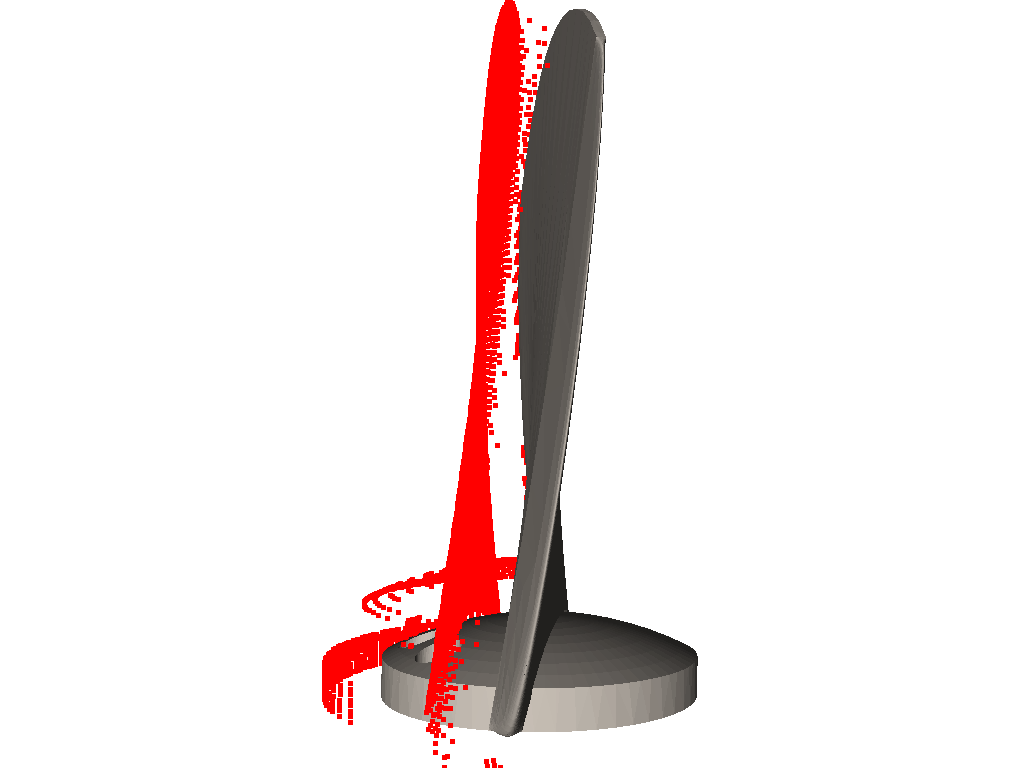
\includegraphics[width=\columnwidth]{figs/bighatch/amostrapa1.png}
	\caption{Pontos amostrados da pá - vista lateral}
	\label{fig::amostrapa1}
\end{figure}

\begin{figure}[h!]	
	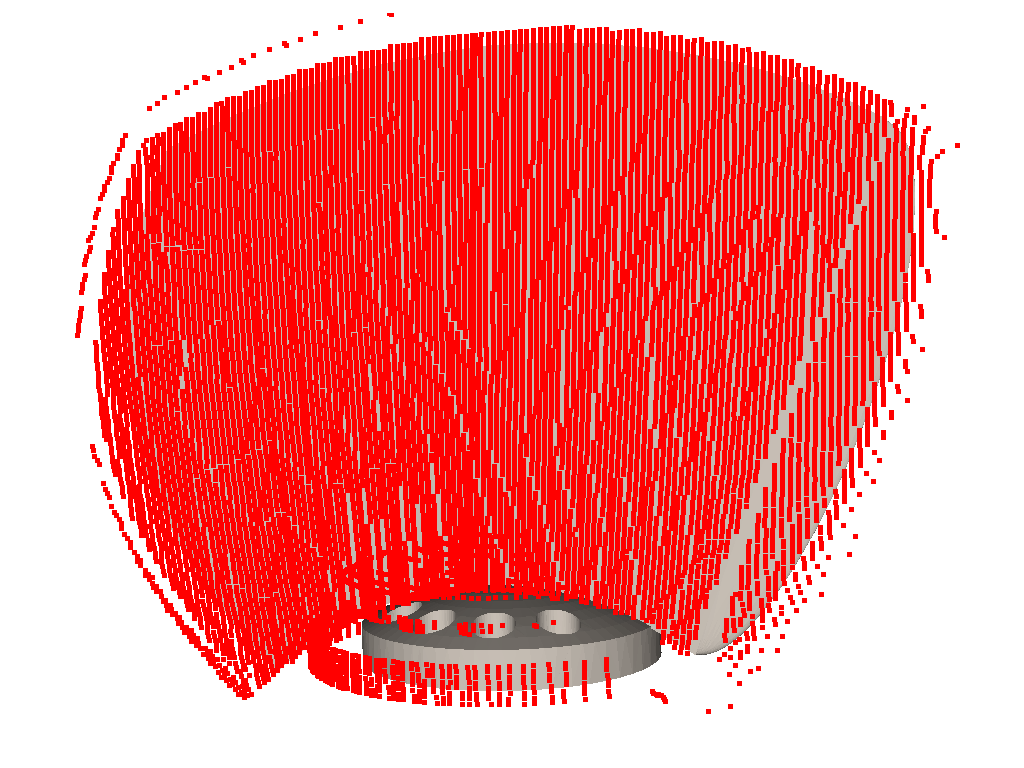
\includegraphics[width=\columnwidth]{figs/bighatch/amostrapa2.png}
	\caption{Pontos amostrados da pá - vista frontal}
	\label{fig::amostrapa2}
\end{figure}

As tabelas~\ref{tab::robocarac} e ~\ref{tab::robocarac} abaixo resume as
caracterísitcas de cada robô e o estudo cinemático realizado, respectivamente:

\begin{center}
\begin{tabular}{  c | c | c | c  }
  \hline
  \textbf{Robô} & \textbf{Payload (Kg)} & \textbf{Massa (Kg)} & \textbf{Alcance
  (mm)} \\ \hline 
  KR10 & 10 & 56 & 1100 \\ \hline
  MH12 & 20 & 130 & 2551  \\ \hline
  LBR 14 & 14 & 30 & 820 \\ \hline
  SIA20D & 20 & 120 &  910 \\
  \hline
\end{tabular}
\captionof{table}{Caracterísitcas principais dos robôs.}
\label{tab::robocarac}
\end{center}

\begin{center}
\begin{tabular}{  c | c | c }
  \hline
  \textbf{Robô} & \textbf{Pontos revestidos (\%)} & \textbf{Posições de base} \\ \hline 
  KR10 & 24.33 & 5\\ \hline 
  MH12 & 53.3 & 2   \\ \hline
  LBR 14 $\uparrow$ & 17.2 & 6 \\ \hline
  LBR 14 $\rightarrow$ & 17.37 & 6 \\ \hline
  SIA20D $\uparrow$ & 23.14 & 5 \\ \hline
  SIA20D $\rightarrow$ & 24.76 & 5 \\ 
  \hline
\end{tabular}
\captionof{table}{Resumo do estudo
cinemático.}
\label{tab::robocin}
\end{center}

\paragraph{KR 10 R1100 sixx WP (Kuka)}
A figura~\ref{fig::kr10cin1} e figura~\ref{fig::kr10cin2} mostram as vistas
lateral e superior do espaço de trabalho do manipulador, respectivamente.

O script que calcula a melhor posição da base em relaçao à pá retornou a posição
870 mm, sendo que 3825 pontos foram revestidos, representando 24.33\% de toda a
pá. Estima-se que serão necessários, pelo menos, 5 posições para o recobrimento
de toda a pá, figura~\ref{fig::kr10bestpos}.



\begin{figure}[h!]	
	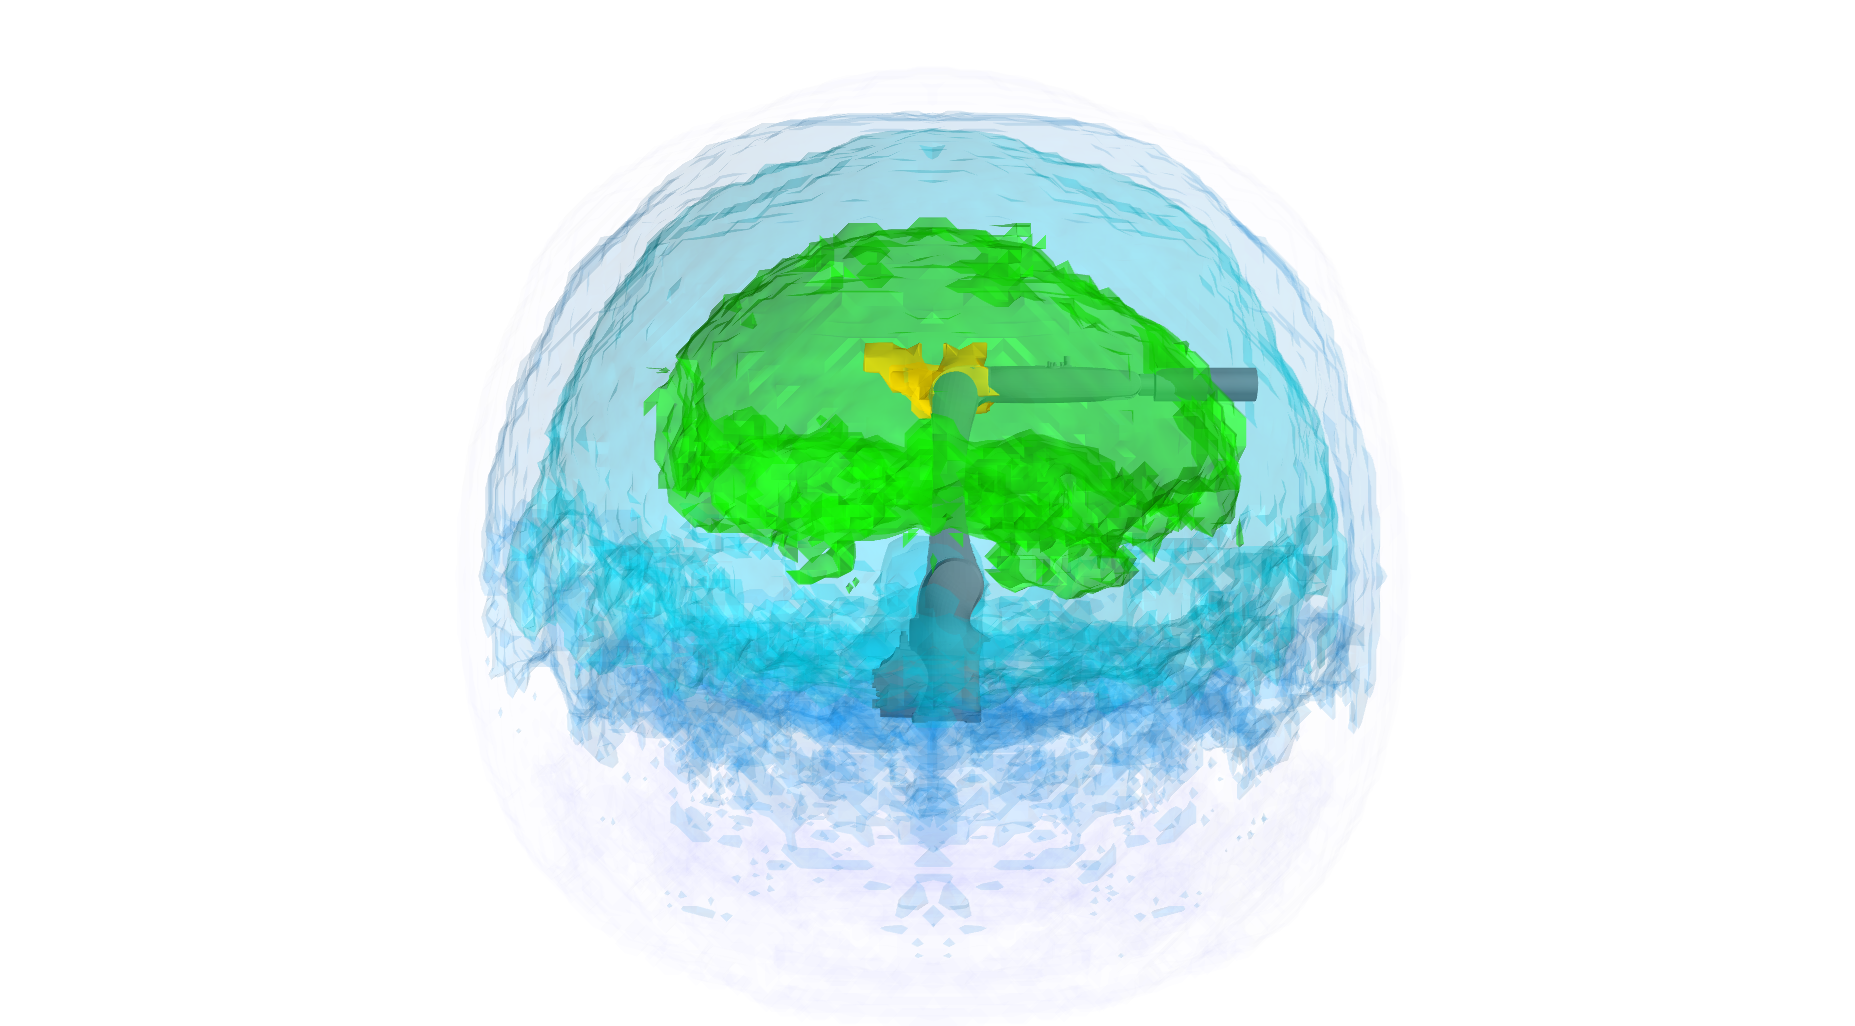
\includegraphics[width=\columnwidth]{figs/bighatch/kr10_front.png}
	\caption{Espaço de trabalho do manipulador Kuka KR10 - vista lateral}
	\label{fig::kr10cin1}
\end{figure}

\begin{figure}[h!]	
	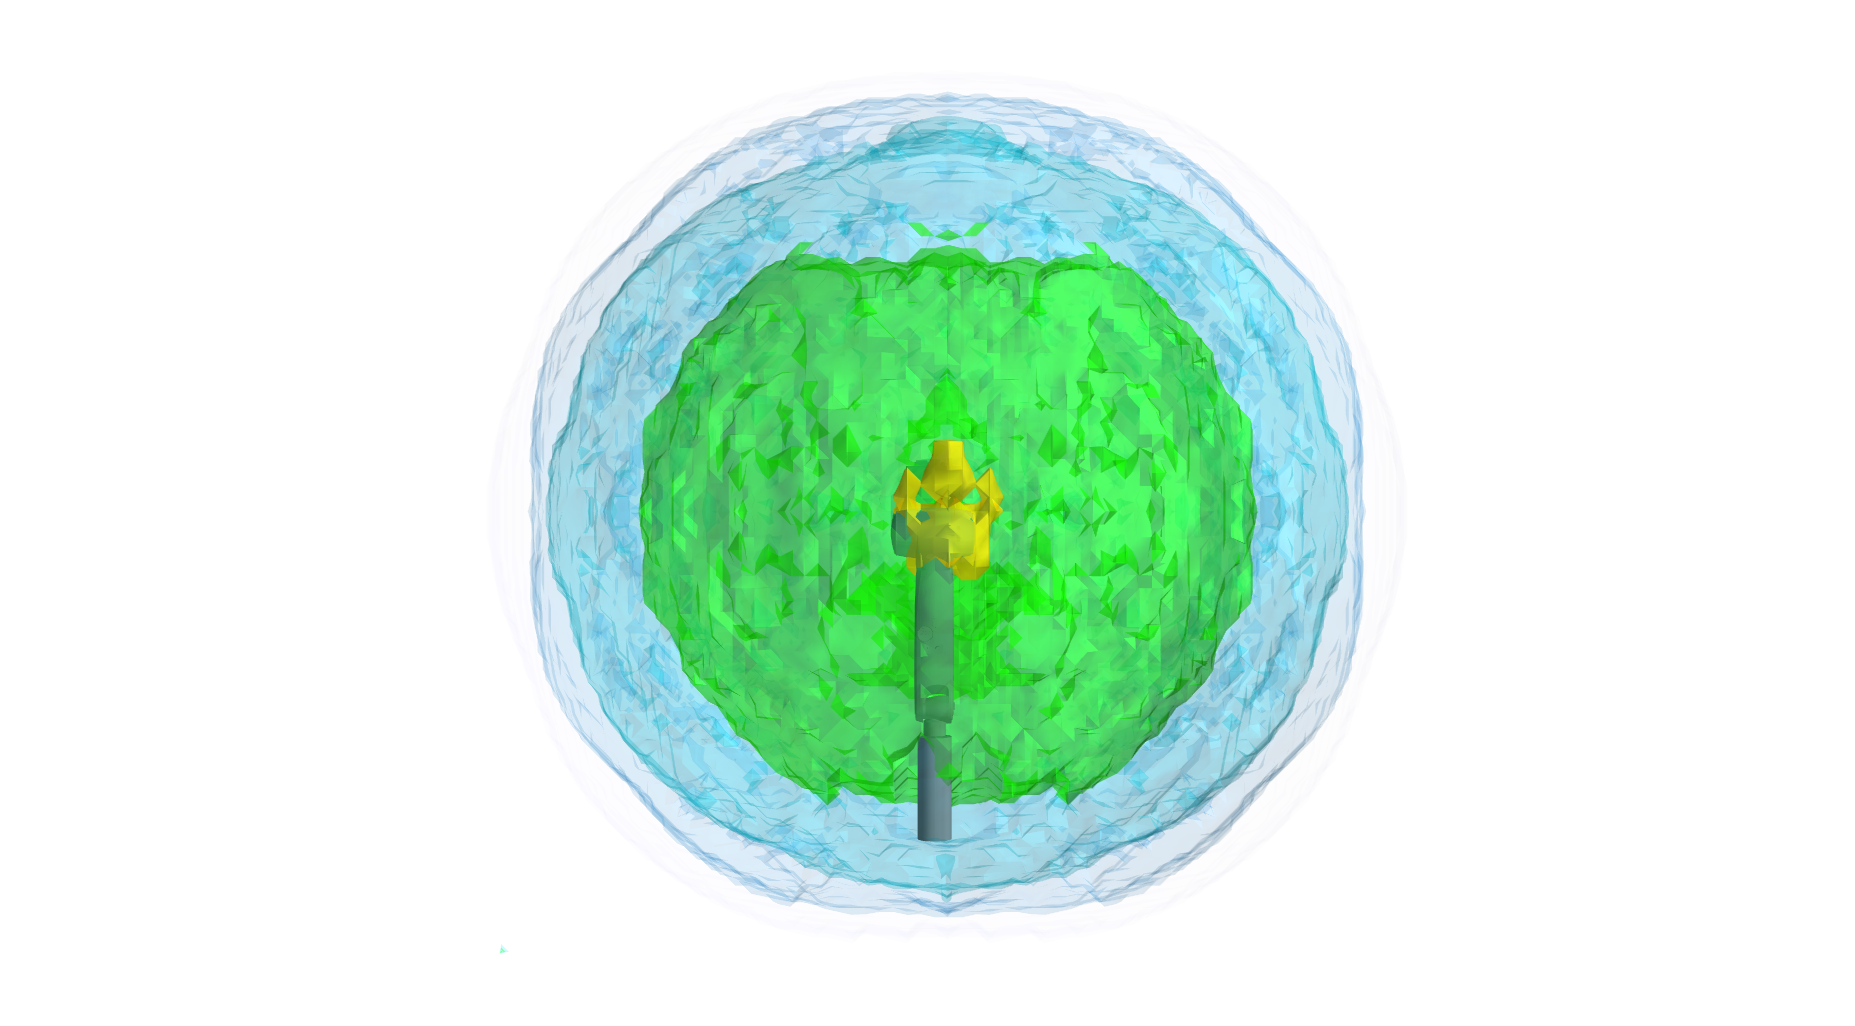
\includegraphics[width=\columnwidth]{figs/bighatch/kr10_top.png}
	\caption{Espaço de trabalho do manipulador Kuka KR10 - vista superior}
	\label{fig::kr10cin2}
\end{figure}

\begin{figure}[h!]	
	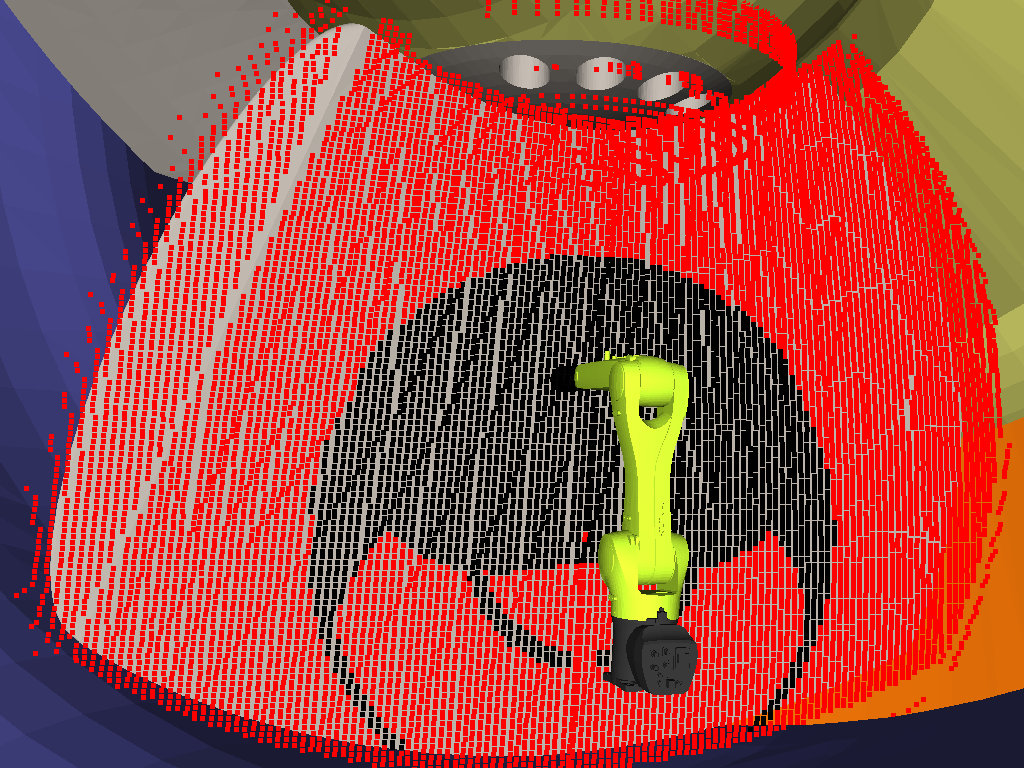
\includegraphics[width=\columnwidth]{figs/bighatch/kr10_bestpos.png}
	\caption{Melhor posição para o revestimento - robô KR10 da Kuka.}
	\label{fig::kr10bestpos}
\end{figure}


\paragraph{MH12 (Motoman)}
A figura~\ref{fig::mh12cin1} e figura~\ref{fig::mh12cin2} mostram as vistas
lateral e superior do espaço de trabalho do manipulador, respectivamente.

O script que calcula a melhor posição da base em relaçao à pá retornou a posição
950 mm, sendo que 8379 pontos foram revestidos, representando 53.30\% de toda a
pá. Estima-se que serão necessários, pelo menos, 2 posições para o recobrimento
de toda a pá, figura~\ref{fig::mh12bestpos}.

\begin{figure}[h!]	
	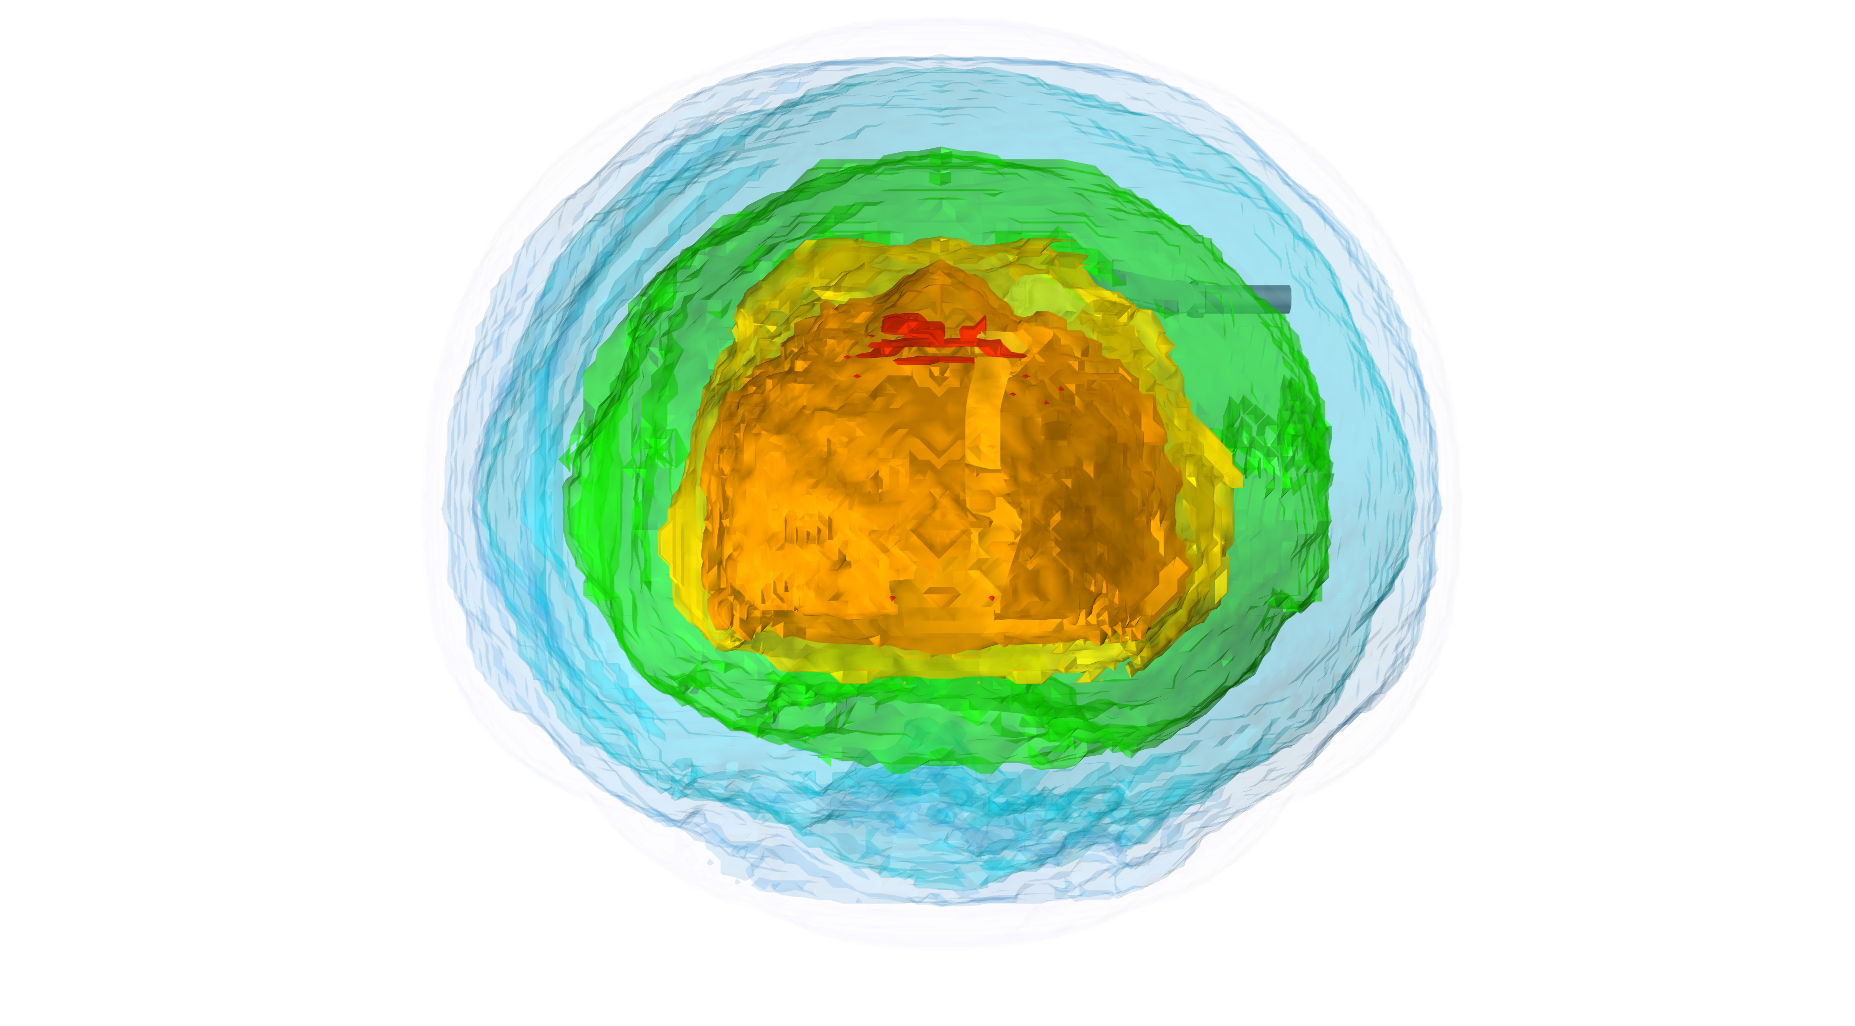
\includegraphics[width=\columnwidth]{figs/bighatch/mh12_front.png}
	\caption{Espaço de trabalho do manipulador MH12 - vista lateral}
	\label{fig::mh12cin1}
\end{figure}

\begin{figure}[h!]	
	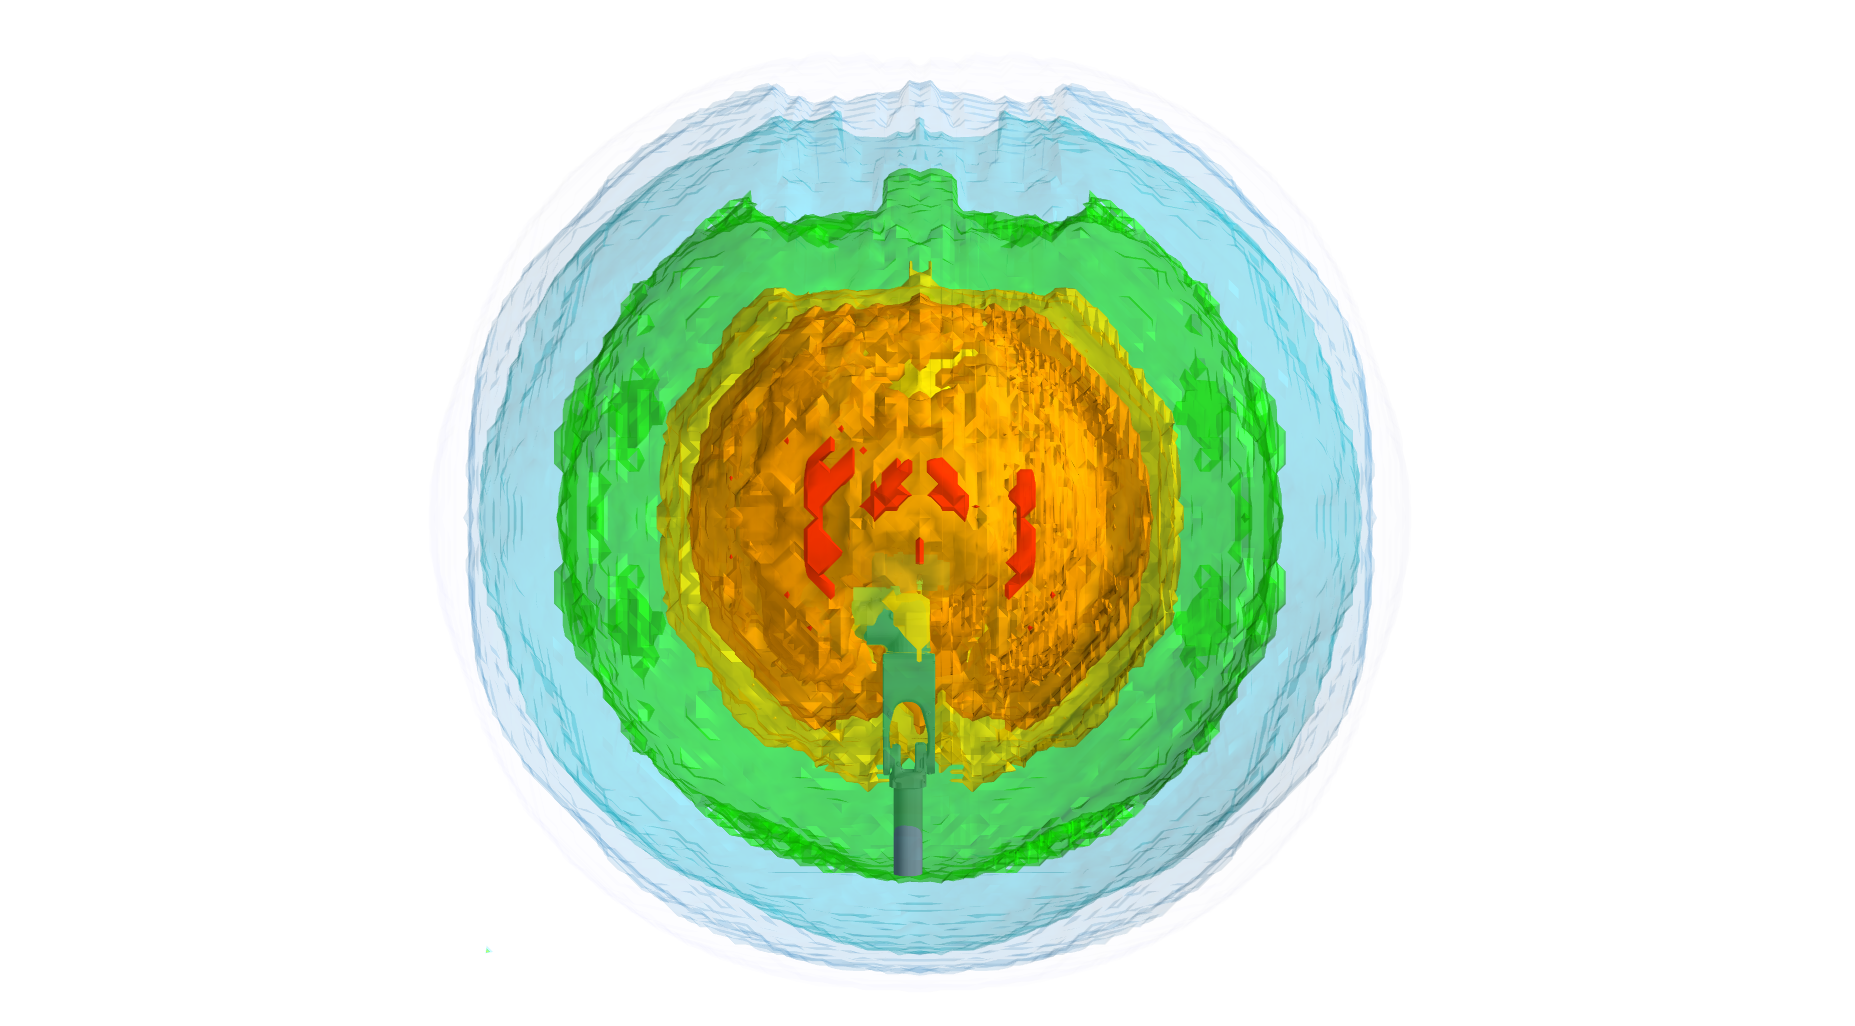
\includegraphics[width=\columnwidth]{figs/bighatch/mh12_top.png}
	\caption{Espaço de trabalho do manipulador MH12 - vista superior}
	\label{fig::mh12cin2}
\end{figure}

\begin{figure}[h!]	
	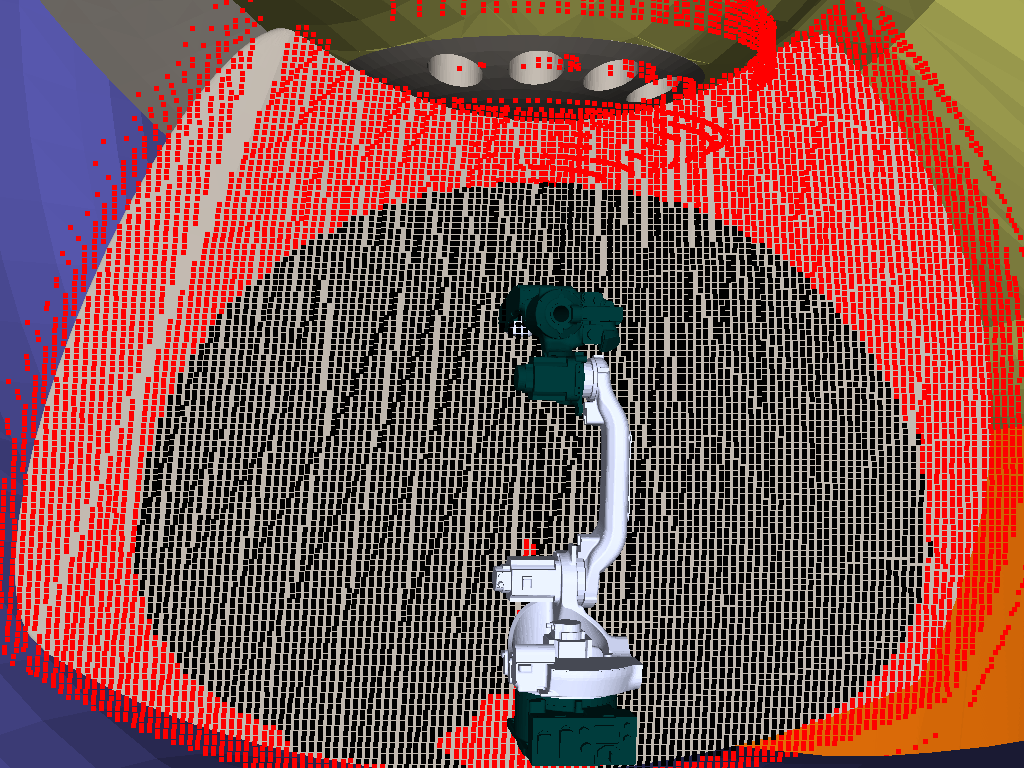
\includegraphics[width=\columnwidth]{figs/bighatch/mh12_bestpos.png}
	\caption{Melhor posição para o revestimento - robô MH12 da Motoman.}
	\label{fig::mh12bestpos}
\end{figure}


\paragraph{LBR iiwa 14 R820 (Kuka)}
O manipulador LBR iiwa 14 R820 possui 7 graus de liberdade e, devido a sua
grande flexibilidade e facilidade de montagem, foram estudadas duas
configurações para a base.

O script que calcula a melhor posição da base na posição vertical em relaçao à
pá retornou a posição 1.06, sendo que 2648 pontos foram revestidos,
representando 17.20\% de toda a pá. Estima-se que serão necessários, pelo menos,
6 posições para o recobrimento de toda a pá, figura~\ref{fig::lbrbestposv}.

\begin{figure}[h!]	
	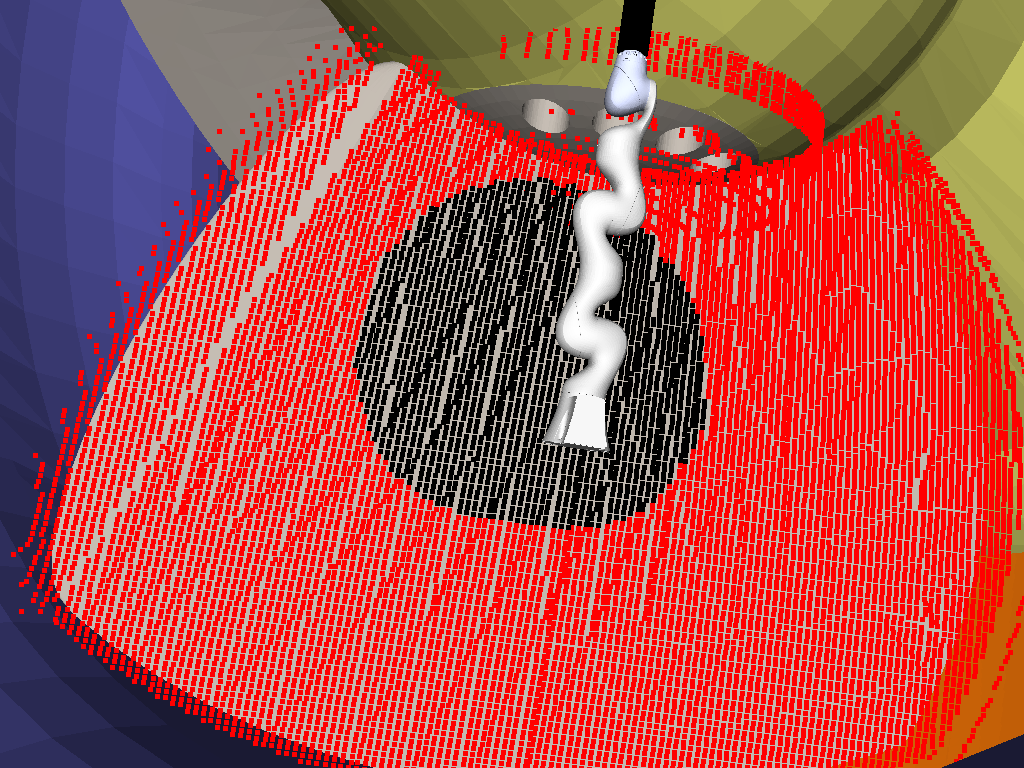
\includegraphics[width=\columnwidth]{figs/bighatch/lbr_bestposv.png}
	\caption{Melhor posição para o revestimento - robô LBR da Kuka com base na
	posição vertical.}
	\label{fig::lbrbestposv}
\end{figure}

O script que calcula a melhor posição da base na posição vertical em relaçao à
pá retornou a posição 1400 mm, sendo que 2730 pontos foram revestidos,
representando 17.37\% de toda a pá. Estima-se que serão necessários, pelo menos,
6 posições para o recobrimento de toda a pá, figura~\ref{fig::lbrbestposh}.

\begin{figure}[h!]	
	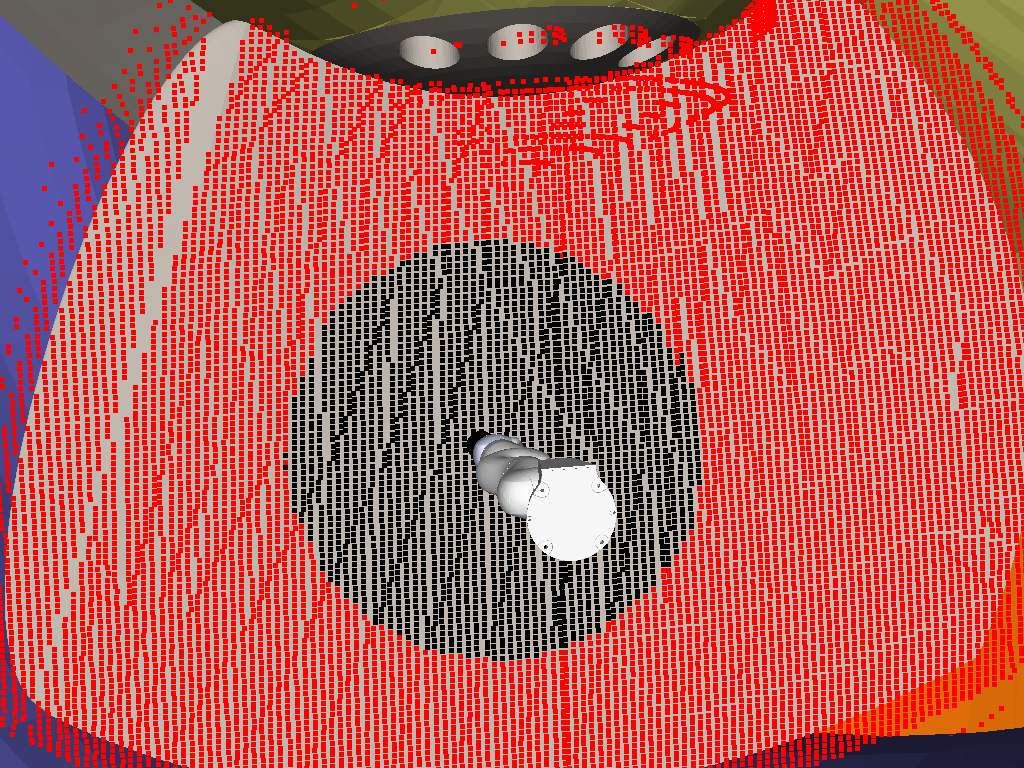
\includegraphics[width=\columnwidth]{figs/bighatch/lbr_bestposh.png}
	\caption{Melhor posição para o revestimento - robô LBR da Kuka com base na
	posição horizontal.}
	\label{fig::lbrbestposh}
\end{figure}

\paragraph{SIA20D (Motoman)}
O manipulador SIA20D também possui 7 graus de liberdade e, devido a sua
grande flexibilidade e facilidade de montagem, foram estudadas duas
configurações para a base.

O script que calcula a melhor posição da base na posição vertical em relaçao à
pá retornou a posição 1100 mm, sendo que 3638 pontos foram revestidos,
representando 23.14\% de toda a pá. Estima-se que serão necessários, pelo menos,
5 posições para o recobrimento de toda a pá, figura~\ref{fig::sia20dbestposv}.

\begin{figure}[h!]	
	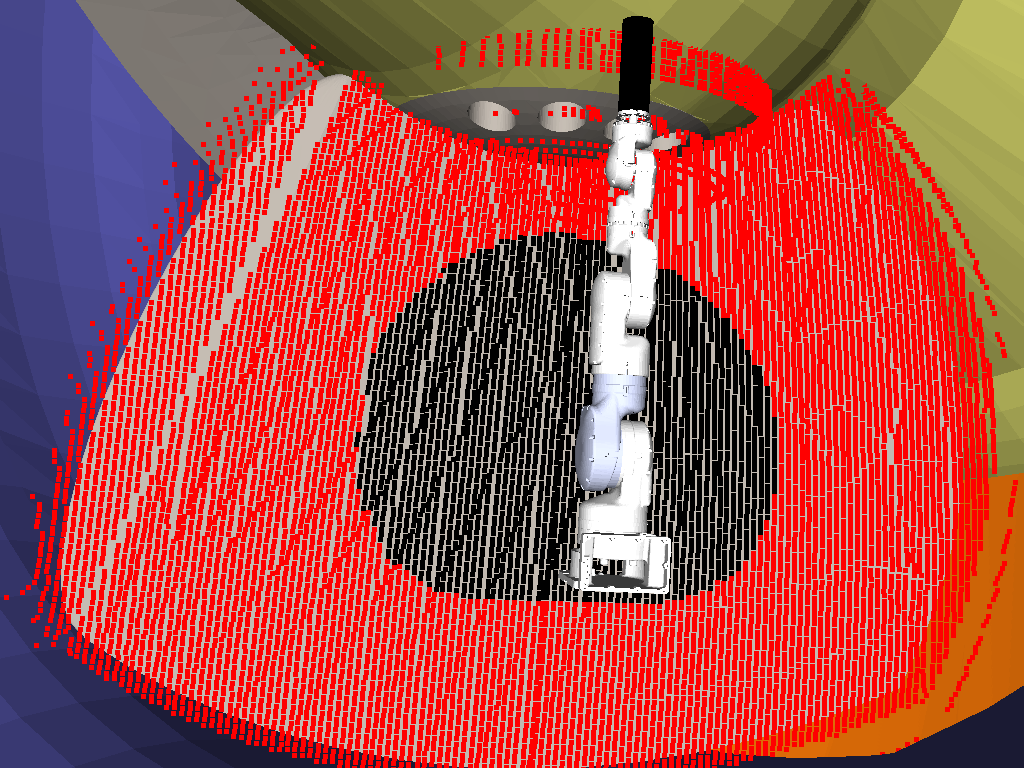
\includegraphics[width=\columnwidth]{figs/bighatch/sia20d_bestposv.png}
	\caption{Melhor posição para o revestimento - robô SIA20D da Motoman com base
	na posição vertical.}
	\label{fig::sia20dbestposv}
\end{figure}

O script que calcula a melhor posição da base na posição horizontal em relaçao à
pá retornou a posição 1510 mm, sendo que 3892 pontos foram revestidos,
representando 24.76\% de toda a pá. Estima-se que serão necessários, pelo menos,
5 posições para o recobrimento de toda a pá, figura~\ref{fig::sia20dbestposh}.

\begin{figure}[h!]	
	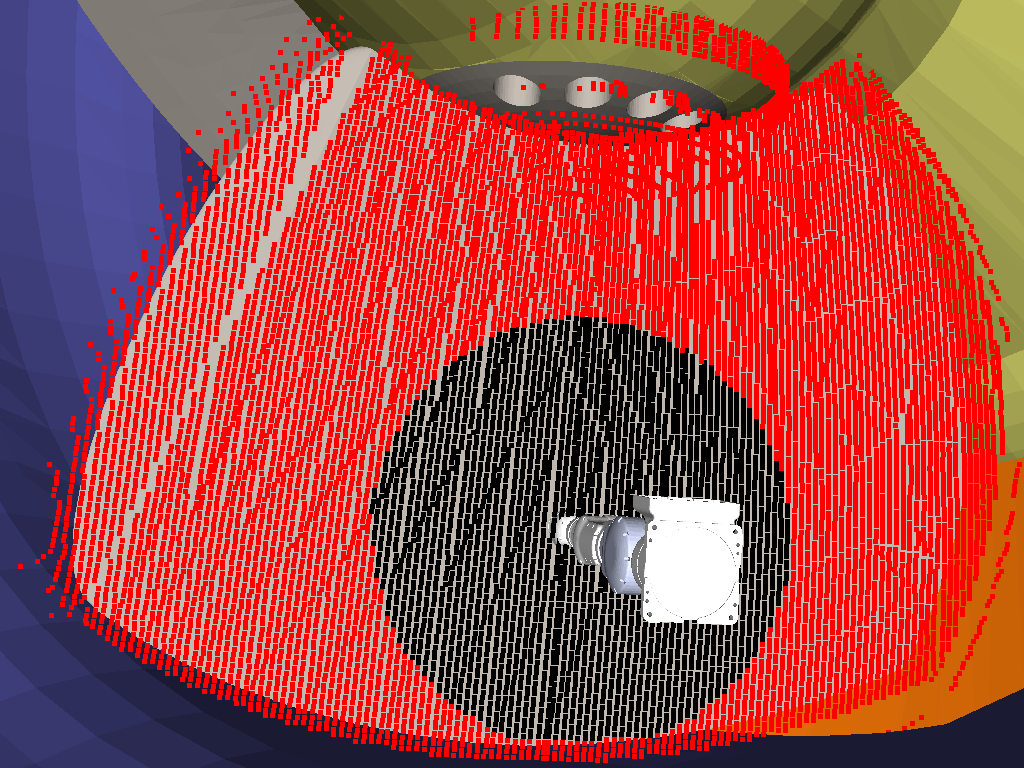
\includegraphics[width=\columnwidth]{figs/bighatch/sia20d_bestposh.png}
	\caption{Melhor posição para o revestimento - robô SIA20D da Motoman com base
	na posição horizontal.}
	\label{fig::sia20dbestposh}
\end{figure}
